\documentclass[handout]{beamer}

\usetheme{Warsaw}

\usepackage[brazil]{babel}
\usepackage[utf8]{inputenc}
\usepackage{times}
\usepackage[T1]{fontenc}
\usepackage{epsfig}
\usepackage{listings}
\usepackage{amsfonts}
\usepackage{multirow}
\usepackage{tikz}
\usepackage{textpos}

%\usepackage{dcolumn}
%\newcolumntype{.}{D{.}{.}{-1}}
%\newcolumntype{d}[1]{D{.}{.}{#1}}
%\usetheme{Berkeley}


\title[Conceitos de Linguagens de Programação]
{%
	Tipos de dados%
}
\author[Prof. Hugo de Paula]
{
	Prof.~Hugo~de~Paula
}
\institute[DCC / PUC Minas]
{
\epsfig{file=puclogo_small_bw,width=1.5cm} \\
  \textsc{Pontifícia Universidade Católica de Minas Gerais}\\
	Departamento de Ciência da Computação
}
\date[]{}

\lstset{language=Java,
        basicstyle=\scriptsize,
        commentstyle=\color{red},
        showstringspaces=false,
        numbers=left,
        literate={á}{{\'a}}1 {ã}{{\~a}}1 {é}{{\'e}}1 {í}{{\'i}}1 {ó}{{\'o}}1 {ú}{{\'u}}1,
        numberstyle=\tiny}

\begin{document}


\selectlanguage{brazil}

\begin{frame}
   \titlepage
\end{frame}

%\addtobeamertemplate{frametitle}{}{%
%	\begin{tikzpicture}[remember picture,overlay]
%	\node[anchor=north east,yshift=2pt] at (current page.north east) {
\epsfig{file=puclogo_small_bw,width=1.2cm}};
%	\end{tikzpicture}}


%\addtobeamertemplate{frametitle}{}{%
	%\begin{tikzpicture}[node distance=0cm, remember picture, overlay, every node/.style={inner sep=0,outer sep=0, node distance=0cm, baseline=0cm}]
	%\node[anchor=north east] at (current page.north east) {
\epsfig{file=puclogo_small_bw,width=1cm}};
	%\end{tikzpicture}}


%\logo{
\includegraphics[height=0.8cm]{puclogo_small_bw.pdf}\vspace{220pt}}


\begin{frame}
   \frametitle{Sumário}
   \tableofcontents[pausesections]
\end{frame}

%\AtBeginSection[] % Do nothing for \section*
%{
%\begin{frame}<beamer>
%\frametitle{Outline}
%\tableofcontents[currentsection]
%\end{frame}}


\addtobeamertemplate{frametitle}{}{%
   \begin{textblock*}{10mm}(.9945\textwidth,-1.89cm)
	   
\includegraphics[height=1cm]{puclogo_small_bw.pdf}
   \end{textblock*}
}



\section{Valores e tipos}

\subsection{Valores e tipos}

\begin{frame}{Valores e tipos}
   \begin{itemize}
   \item \textbf{Valor}: tudo aquilo que pode ser avaliado, armazenado, e passado como parâmetro
		\begin{itemize}
			\item Valores são agrupados em tipos
		\end{itemize}
   \item \textbf{Tipo}: conjunto de valores e de operações que podem ser realizadas sobre os mesmos
		\begin{itemize}
			\item \textit{Matematicamente}: baseados na teoria dos conjuntos
			\item \textit{Computacionalmente}: definem também quantidade de memória e forma de codificação
				\begin{itemize}
					\item Na matemática: $\mathbb{Z} = [-\infty,+\infty]$
					\item Em computação: $int = [MIN\_INT, MAX\_INT]$
				\end{itemize}
		\end{itemize}
		\item Linguagens de Programação devem incluir um conjunto de entidades que representam tipos de dados simples e prover mecanismos para a construção de novos tipos (abstração de dados)
		\item Tipos podem ser: primitivos, compostos e recursivos
   \end{itemize}
\end{frame}

\subsection{Tipos primitivos}

\begin{frame}[fragile]{Tipos primitivos}
   \begin{itemize}
   \item \textbf{Tipo primitivos}:
      \begin{itemize}
      \item Valores são atômicos (não decomponíveis)
      \item Exemplos: inteiros, reais, caractere, lógicos, enumerados
			\end{itemize}
	\item Tipos pré-definidos: tipos fornecidos pela LP, a partir dos quais todos os outros tipos são construídos
		\begin{itemize}
		\item Normalmente identificados por palavras reservadas da linguagem
		\end{itemize}
  \end{itemize}

\begin{block}{Exemplo: Tipos primitivos do Pascal}
\scriptsize
\centering
    \begin{tabular}{rrp{3.8cm}p{3.8cm}}
    \hline
    \textbf{Tipo} & \textbf{\textit{sizeof()}} & \textbf{Descrição} \\
    \hline
    \textbf{char}    &   8-bit     & codificação ASCII \\
    \textbf{integer} &  16/32-bit  & número inteiro (tamanho pode variar com a implementação) \\
    \textbf{real}    &   32-bit    & número real \\
    \textbf{boolean} &   1-bit     & tipo lógico (true, false) \\
    \hline
    \end{tabular}%
\end{block}

\end{frame}

\begin{frame}[fragile]{Exemplos de tipos primitivos pré-determinados}
\begin{block}{Exemplo: Tipos primitivos do Java}
\scriptsize
\centering
    \begin{tabular}{rrrr}
    \hline
    \textbf{Tipo} & \textbf{\textit{sizeof()}} & \textbf{Valor mínimo} & \textbf{Valor Máximo} \\
    \hline
    \textbf{char} &   16-bit   &   Unicode $0$ &   Unicode $2^{16}-1$ \\
    \textbf{byte} &   8-bit   &   $-128$ &   $+127$ \\[1mm]
    \multirow{2}[2]{*}{\textbf{short}} & \multirow{2}[2]{*}{  16-bit  } &   $-2^{15}$ &   $+2^{15}-1$ \\[1mm]
																			 &      						 							& $-32,768$ &   $-32,767$ \\[1mm]
    \multirow{2}[2]{*}{\textbf{int}} & \multirow{2}[2]{*}{  32-bit  } 	&   $-2^{31}$ &   $+2^{31}-1$ \\[1mm]
																			 &					 							& \tiny $-2,147,483,648$ & \tiny $2,147,483,647$ \\[1mm]
    \multirow{2}[2]{*}{\textbf{long}} & \multirow{2}[2]{*}{  64-bit  } &   $-2^{63}$ &   $+2^{63}-1$ \\[1mm]
          &       & \tiny $-9,223,372,036,854,775,808$ & \tiny $9,223,372,036,854,775,807$ \\[1mm]
    \textbf{float} &   32-bit   & \multicolumn{2}{l}{32-bit IEEE 754 floating-point numbers}  \\[1mm]
    \textbf{double} &   64-bit   & \multicolumn{2}{l}{64-bit IEEE 754 floating-point numbers} \\[1mm]
    \textbf{bool} &   1-bit   & \multicolumn{2}{l}{true or false} \\[1mm]
    \textbf{void} &   -----   &   -----   &   -----   \\
    \hline
    \end{tabular}%
\end{block}
\end{frame}


\begin{frame}[fragile]{Tipos primitivos: tipo complexo}

\begin{block}{Número complexo}
    Matematicamente, um número é escrito na sua forma $a + b\jmath$. Os elementos $a$ e $b$ são números reais em que o valor de $a$ representa a parte real e o valor de $b$ representa a parte imaginária de um número complexo.
\end{block}

\begin{itemize}
    \item Algumas linguagens suportam o número complexo como um tipo primitivo, apesar de possuir partes ``decomponíveis''. Ex: Fortran, Python e C99.
    \item Cada valor é representado por dois elementos \lstinline|float|.
    \item Forma literal no Python: \lstinline|(10 + 2j)|.
\end{itemize}

\end{frame}


\begin{frame}[fragile]{Tipos primitivos: \lstinline|boolean| (lógico)}

\begin{itemize}
    \item Apenas dois elementos: \lstinline|true| e \lstinline|false|.
    \item Pode ser implementado como bit, mas normalmente é implementado como byte.
    \item Possui operações lógicas associadas: conjunção (AND, \verb!&&!, $*$), disjunção (OR, \verb!||!, +) e negação (NOT, \lstinline|!|, $\tilde{{}}$), ou exclusivo (XOR, \verb|^|).
    \item Mas operações relacionais sobre tipos numéricos também produzem valores lógicos: $>, <, \leq, \geq, \equiv, \neq$.
    \item Linguagem C usa inteiros para representar valores lógicos: 0 (\lstinline|false|), $\neq 0$ (\lstinline|true|).
\end{itemize}

\end{frame}

\begin{frame}[fragile]{Tipos primitivos: strings}

\begin{itemize}
    \item Questões polêmicas de projeto:
    \begin{itemize}
        \item Deve ser um tipo primitivo ou uma cadeia de caracteres?
        \item Devem possui comprimento estático ou dinâmico?
    \end{itemize}
    \item Operações típicas: atribuição, cópia, comparação, concatenação, referência para substring e casamento de padrões.
    \item Strings estáticas: Java (classe \lstinline|String|)
    \item String dinâmicas de comprimento limitado: C e C++. Utilizam um caractere especial que indicam o final da string (ex.: \textit{nulll terminated string}).
    \item Strings dinâmicas: Perl e JavaScript. Não possuem máximo.
\end{itemize}

\end{frame}

\begin{frame}[fragile]{Tipos primitivos: strings}
\begin{center}
\begin{tabular}{p{5cm}p{5cm}}
\multicolumn{1}{c}{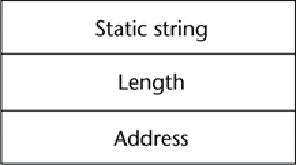
\includegraphics[width=4cm]{figuras/stringestatica.pdf}}    &
\multicolumn{1}{c}{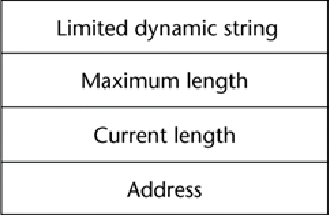
\includegraphics[width=4cm]{figuras/stringdinamica.pdf}} \\
Descritor de strings estáticas em tempo de compilação. &
Descritor de strings dinâmicas de comprimento limitado em tempo de execução. \\
\end{tabular}
\end{center}



\end{frame}

\subsubsection{Tipos enumerados}

\begin{frame}[fragile]{Construtores de tipos primitivos: tipos enumerados}
   \begin{itemize}
			\item \textbf{Tipos Enumerados}: conjuntos cujos elementos são listados e enumerados explicitamente
			\item Na maioria das linguagens o conjunto é ordenado (ou seja, a ordem de enumeração é importante)
			\item Operadores mais comuns são sucessor e antecessor
	\end{itemize}
\begin{block}{Exemplo em C++ / C}
	\begin{lstlisting}[language=C,numbers=none]
         enum dia_semana {dom, seg, ter, qua, qui, sex, sab};
         dia_semana hoje, ontem;
         ontem = seg;
         hoje = ontem + 1;

         enum cores { vermelho = 1, verde = 256, azul = 65536};
	\end{lstlisting}
\end{block}
\end{frame}


\begin{frame}[fragile]{Construtores de tipos primitivos: tipos enumerados}
\begin{block}{Exemplo em Pascal}
	\begin{lstlisting}[language=Pascal,numbers=none]
     type
          Dia = ( seg, ter, qua, qui, sex, sab, dom )

     var
          hoje, amanha : Dia;

     begin
          hoje := seg;
          if  ( hoje  =   ter ) ...
          amanha := succ(hoje);
     end.
	\end{lstlisting}
\end{block}

\end{frame}


\subsubsection{Tipos subfaixa}

\begin{frame}[fragile]{Construtores de tipos primitivos: tipos subfaixa}
   \begin{itemize}
			\item \textbf{Tipos subfaixa}: subconjuntos de tipos primitivos cujos elementos são especificados
			definido o limite inferior e o limite superior dos elementos (intervalo)
	\end{itemize}

\begin{block}{Exemplo em Pascal}
	\begin{lstlisting}[language=Pascal,numbers=none]
     type
          Dias_do_Mes    = 1..30;
          unsigned_byte  = 0..255;
          signed_byte    = -128..127;
          string         = packed array [1..255] of char;
     var
          x : 1..10;
          y : 'a'..'z';
	\end{lstlisting}
\end{block}

   \begin{itemize}
			\item C e Java não suportam tipos subfaixa, mas o seu comportamento pode ser simulado com \textit{Iterators}
	\end{itemize}

\end{frame}


\subsection{Tipos compostos}

\begin{frame}{Tipos compostos}

   \begin{itemize}
		\item Valores são compostos a partir de valores mais simples
		\item Uma vez que tipos são conjuntos, operações sobre conjuntos podem ser utilizadas para construir novos tipos a partir dos tipos existentes (abstrações de tipos de dados)
		\item Essas operações são chamadas de construtores de tipos

   \item Construtores de tipos compostos:
      \begin{itemize}
      \item Produto Cartesiano, União Disjunta, Mapeamento, Conjunto Potência
      \end{itemize}
	\end{itemize}
\end{frame}

\begin{frame}[fragile]{Tipo ponteiro}
\begin{itemize}
    \item Um tipo ponteiro possui uma faixa de valores que corresponde a endereços de memória, e um valor especial \textit{nil} (normalmente representado pelo zero).
    \item Provê endereçamento indireto.
    \item Usado para gerenciamento dinâmico de memória.
    \item Região de memória em que o armazenamento é criado dinamicamente é chamado de \textit{heap}.
    \item Tipo do ponteiro indica forma de codificação da região apontada.
    \item Em C: ponteiro \lstinline|void| pode apontar para região de qualquer tipo.
\end{itemize}
\end{frame}

\begin{frame}[fragile]{Tipo ponteiro}
\begin{itemize}
    \item Operações fundamentais: atribuição e dereferenciação.
    \begin{itemize}
        \item Atribuição: direciona o ponteiro para um endereço de memória.
        \item Dereferenciação: retorna o valor armazenado no local apontado pelo valor do ponteiro.
    \end{itemize}
\begin{center}
    \item Ex. em C:

\begin{tabular}{lll}
    \hline
    \textbf{Declaração} & \textbf{Semântica} & \textbf{Semântica} \\
     & \textbf{de valor} & \textbf{de referência} \\ \hline
     \lstinline|int i| & \lstinline|i| & \lstinline|&i| \\
     \lstinline|int *ptr| & \lstinline|*ptr| & \lstinline|ptr| \\
     \lstinline|int fun()| & \lstinline|fun()| & \lstinline|fun| \\
     \hline
\end{tabular}
\end{center}

\end{itemize}


\end{frame}


\subsubsection{Produto cartesiano}

\begin{frame}{Produto cartesiano}
		\begin{itemize}
			\item \textit{Matematicamente}: $A \times B = \left\{ (x, y) | x \in A, y \in B \right\}$
				\begin{itemize}
					\item O produto cartesiano de $n$ conjuntos $S_1, S_2, \ldots, S_n$,
				denotado por $S_1 \times S_2 \times \ldots \times S_n$, é um conjunto cujos elementos são \textit{n-tuplas} ordenadas, onde $s_i \in S_i$
				\end{itemize}

			\item \textit{Computacionalmente}: São vistos por linguagens de programação como campos com nomes simbólicos: tuplas, registros, estruturas.
				\begin{itemize}
					\item Diferença entre produto cartesiano e um registro:
					\begin{itemize}
						\item No registro, os campos possuem nomes
						\item No produto cartesiano, os campos são identificados pela sua posição
					\end{itemize}
				\end{itemize}
		\end{itemize}
 \end{frame}

\begin{frame}[fragile]{Produto cartesiano}

\begin{block}{Exemplo em C++ }
	\begin{lstlisting}[language=C,numbers=none]
      typedef struct {
          int dia;
          int mes;
          int ano;
      } Data;

      Data natal;

      natal.dia = 25;
      natal.mes = 12;
      natal.ano = 00;
	\end{lstlisting}
\end{block}

\begin{itemize}
	\item Na Programação Orientada para Objetos, as classes são formas de implementação de produtos cartesianos
\end{itemize}

\end{frame}


\begin{frame}[fragile]{Produto cartesiano}

\begin{block}{Exemplo em Pascal}
	\begin{lstlisting}[language=Pascal,numbers=none]
     type
          Data = record
               dia : integer;
               mes : integer;
               ano : integer;
          end;

     var
          natal :  Data;

     begin
          natal.dia := 25;
          natal.mes := 12;
          natal.ano := 00;
     end.
	\end{lstlisting}
\end{block}


\end{frame}



\begin{frame}{Produto cartesiano}
		\begin{itemize}
			\item Memória:
				\begin{itemize}
					\item $\mathrm{sizeof}(A \times B) = \mathrm{sizeof}(A) + \mathrm{sizeof}(B)$
				\end{itemize}

			\item Cardinalidade:
				\begin{itemize}
					\item $\sharp(A \times B) = \sharp A  \times \sharp B$
				\end{itemize}

			\item Exemplo do registro \textbf{Data}, considerando que o tipo \textit{int} possui 4 bytes
				\begin{itemize}
					\item $Data = int \times int \times int$
					\item $sizeof(Data) = sizeof(int) + sizeof(int) + sizeof(int) = 12\; bytes$
					\item $\sharp Data = 2^{32} \times 2^{32} \times 2^{32} = 2^{96}$
				\end{itemize}
		\end{itemize}
 \end{frame}

\begin{frame}[fragile]{Tipo de dados Registro}

	\begin{block}{Estrutura típica de um tipo de dados Registro}
		\centering
    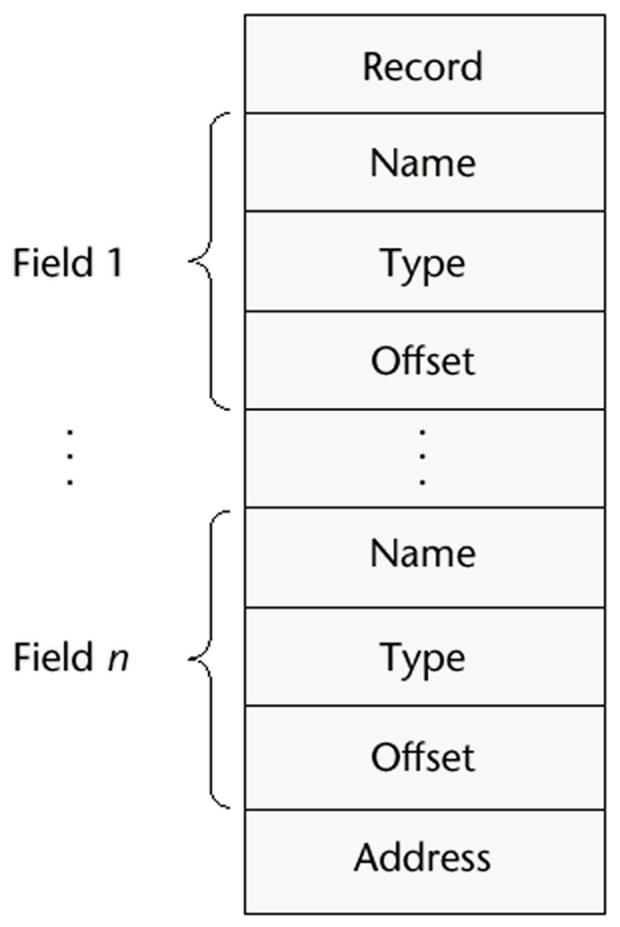
\epsfig{file=figuras/registro,width=3.8cm}
    \end{block}

\end{frame}


\subsubsection{União disjunta}

\begin{frame}{União}
   \begin{itemize}
			\item Estrutura cujos campos compartilham uma área de memória.

			\item \textit{Matematicamente}: $A + B = \left\{ x | x \in A\, \mathrm{ou}\, x \in B \right\}$

			\item \textit{Computacionalmente}: Implementa-se união disjunta. Mesmo que dois conjuntos possuam valores análogos, os valores do tipo A serão sempre considerados distintos dos valores do tipo B.
				\begin{itemize}
					\item Exemplo: Seja $T = \{ a, b, c\}$, então $ T + T =\{ esq\, a, esq\, b, esq\, c, dir\, a, dir\, b, dir\, c \} \neq T$
					\item Na matemática $T \cup T = T$,
				\end{itemize}
		\end{itemize}
\end{frame}



\begin{frame}[fragile]{União livre}
\begin{itemize}
	\item C/C++, cria uma união não discriminada.
    \item União livre é \textbf{unsafe}, pois não permite checagem de tipos.
\end{itemize}

\begin{block}{Exemplo de união livre em C++ }
	\begin{lstlisting}[language=C,numbers=none]
   enum tipo_dados {inteiro, real, logico};
   struct Constante {
      char *nome;  tipo_dados  tipo;
      union {             // valor_int, valor_real e
          int val_int;    // valor_log compartilham a
          float val_real; // mesma área de memória
          bool val_log;   // tam. da área = sizeof(float)
      } valor;
   };
   Constante c;
   strcpy(c.nome,"pi"); c.tipo = real;
   c.valor.val_real = 3.1415926;
	\end{lstlisting}
\end{block}

\end{frame}


\begin{frame}[fragile]{União discriminada}

   \begin{itemize}
		\item Em Pascal: registro variante
   \end{itemize}
\begin{block}{Exemplo de união discriminada em Pascal }
	\begin{lstlisting}[language=Pascal,numbers=none]
   type
      Cores= (vermelho, verde, azul);
      Formas= (circulo, triangulo, retangulo);
      Figura = record
         preenchida: boolean;
         cor: Cores;
         case tipo: Formas of   { tag ou discriminante }
              circulo:    (diametro: real);
              triangulo:  (lado: real; altura: real);
              retangulo:  (lado1: real; lado2: real);
         end
      end;
	\end{lstlisting}
\end{block}

\end{frame}



\begin{frame}{União disjunta}
		\begin{itemize}
			\item Memória:
				\begin{itemize}
					\item $\mathrm{sizeof}(A + B) = max(\mathrm{sizeof}(A),\mathrm{sizeof}(B))$
				\end{itemize}

			\item Cardinalidade:
				\begin{itemize}
					\item $\sharp(A + B) = \sharp A + \sharp B$
				\end{itemize}

			\item Uniões são úteis para reduzir a alocação de memória quando diferentes dados não são necessários simultaneamente
			\item Uniões não são necessárias em linguagens orientadas para objeto: pode-se utilizar herança
			\begin{itemize}
				\item Em C\#, no entanto, é possível se simular união com \textit{StructLayout}
			\end{itemize}

		\end{itemize}
 \end{frame}

\begin{frame}[fragile]{União disjunta}

\begin{block}{Exemplo em C\# de StructLayout }
	\begin{lstlisting}[language=c++,numbers=none]
     using System.Runtime.InteropServices;

     [StructLayout(LayoutKind.Explicit)]

     struct UniaoSimulada {
          [FieldOffset(0)]
          public byte val_byte;
          [FieldOffset(0)]
          public int val_int;
          [FieldOffset(0)]
          public float val_float;
     }
	\end{lstlisting}
\end{block}

\end{frame}



\subsubsection{Mapeamento}

\begin{frame}[fragile]{Mapeamento}

\begin{itemize}
   \item \textit{Matematicamente}: $m: A \rightarrow B = \left\{ y = f(x) | x \in A, y \in B \right\}$
	 \item Um mapeamento é uma função de um conjunto finito de valores A em valores de um tipo B.
   \item Mapeamentos em LP: implementados de duas formas
   \begin{itemize}
       \item Por meio de arranjos.
       \item Por meio de abstrações de função.
   \end{itemize}
\end{itemize}
\end{frame}


\begin{frame}[fragile]{Mapeamento: arranjos}


\begin{block}{Exemplo em C}
	\begin{lstlisting}[language=c,numbers=none]
     bool impar[10] = {0, 1, 0, 1, 0, 1, 0, 1, 0, 1};
  \end{lstlisting}
\end{block}
  \begin{itemize}
		\item Um arranjo representa um  mapeamento finito, onde o conjunto do índice é enumerável.
		\item Muitas linguagens possuem arranjos multidimensionais.
		\item O conjunto do índice deve ser discreto.
  \end{itemize}
\end{frame}



\begin{frame}[fragile]{Mapeamento: arranjos}

\begin{block}{Exemplo em Pascal}
	\begin{lstlisting}[language=Pascal,numbers=none]
     type
         matriz = array [1..10, 0..20] of integer;
     var
         impar : array [1..100] of Boolean;
   \end{lstlisting}
\end{block}

\begin{itemize}
   \item Matematicamente:
   \begin{itemize}
      \item $\mathrm{matriz}: [1; 10]\, \times\, [0; 20] \rightarrow \mathbb{Z}$
      \item $\mathrm{impar}: [1; 100] \rightarrow \{V; F\}$
   \end{itemize}
\end{itemize}

\end{frame}

\begin{frame}[fragile]{Mapeamento: arranjos}
\begin{itemize}
    \item Tipos dos índices dos arranjos:
    \begin{itemize}
        \item Fortran e C: apenas int.
        \item Java: tipos inteiros (byte, short, int long, unsigned int, etc..)
    \end{itemize}
    \item Verificação de índice fora da faixa:
    \begin{itemize}
        \item Fortran, C, Perl: Não verificam faixa dos índices.
        \item Java, C\#: especificam checagem de faixa de índice.
    \end{itemize}
\end{itemize}
\end{frame}

\begin{frame}[fragile]{Variáveis Arranjos}

\begin{itemize}
    \item Quando o conjunto de índices de um arranjo é determinado?

    \item Arranjos Estáticos:
    \begin{itemize}
        \item Conjunto de índices determinado em tempo de compilação
        \item Exemplos: Pascal e C++
    \end{itemize}
\end{itemize}
\begin{block}{Exemplo em Pascal}
    \begin{lstlisting}[language=Pascal,numbers=none]
    var
    vetor : array [1..10] of integer;
    \end{lstlisting}
\end{block}
\end{frame}


\begin{frame}[fragile]{Variáveis Arranjos}
\begin{itemize}
\item Arranjos Dinâmicos:
\begin{itemize}
    \item Conjunto de índices determinado em tempo de execução, no momento da criação do arranjo
    \item Uma vez determinado, conjunto de índices não pode ser alterado
    \item Exemplo: Java
\end{itemize}
\end{itemize}
\begin{block}{Exemplo em Java}
\begin{lstlisting}[language=Java,numbers=none]
int [] x;
int y = Console.readInt();
x = new int [y];
\end{lstlisting}
\end{block}
\end{frame}



\begin{frame}[fragile]{Variáveis Arranjos}
\begin{itemize}
\item Arranjos Flexíveis:
\begin{itemize}
\item Conjunto de índices  pode variar durante a execução
\item Exemplo: Perl
\end{itemize}
\end{itemize}

\begin{block}{Exemplo em Perl}
\begin{lstlisting}[language=Perl,numbers=none]
@fib = ();
@fib = (0, 1, 1, 2, 3, 5);
@fib = (0, 1, 1, 2, 3, 5, 8, 13, 21, 34);
\end{lstlisting}
\end{block}
\end{frame}


\begin{frame}[fragile]{Variáveis Arranjos}
\begin{itemize}
\item Arranjos Flexíveis em Bash:
\begin{itemize}
\item Conjunto de índices não precisa ser consecutivo ou contínuo
\item Partes do vetor não precisam ser inicializadas
\end{itemize}
\end{itemize}

\begin{block}{Exemplo em Bash}
\begin{lstlisting}[language=Bash,numbers=none, basicstyle=\tiny]
area[13]=10
area[32]=TEXTUAL

echo "area[13] = ${area[13]}"
echo "Conteúdo de area[32] é ${area[32]}."

echo -n "area[46] = "
echo ${area[46]}         # não imprime nada

for i in "${area[@]}"; do
echo "${i}"
done
\end{lstlisting}
\end{block}
\end{frame}



\begin{frame}[fragile]{\textit{Slices} (fatiamento)}

\begin{block}{Slice}
    Uma fatia (\textit{slice}) é uma subestrutura de um arranjo. Serve como mecanismo de referenciação.
\end{block}

\begin{itemize}
    \item Úteis quando a linguagem provê operações sobre arranjos.
    \item Ex: Python
\end{itemize}
\begin{lstlisting}[language=Python,numbers=none]
vetor = [2, 4, 6, 8, 10, 12, 14, 16]
matriz = [[1, 2, 3], [4, 5, 6], [7, 8, 9]]

vetor(3:6) % é um arranjo de 3 elementos.
mattriz[0][0:2] % 2 primeiros elementos da 1a linha da matriz.

\end{lstlisting}
\end{frame}


\begin{frame}[fragile]{Descritores de arranjos}

\begin{center}
    \begin{tabular}{p{5cm}p{5cm}}
        \multicolumn{1}{c}{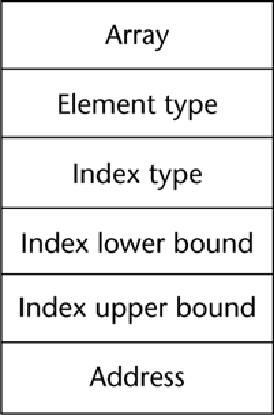
\includegraphics[width=3cm]{figuras/arranjo1d.pdf}}    &
        \multicolumn{1}{c}{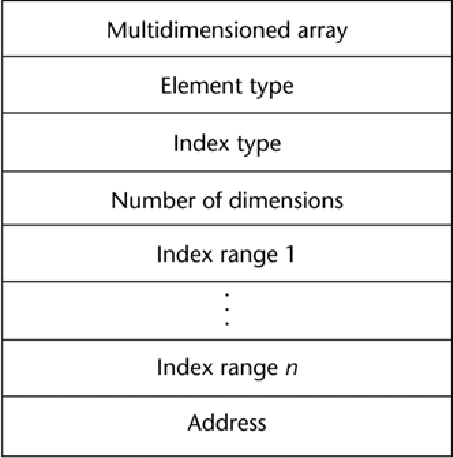
\includegraphics[width=4.5cm]{figuras/arranjond.pdf}} \\
        Descritor de arranjo 1-D em tempo de compilação. &
        Descritor de arranjo N-D em tempo de compilação. \\
    \end{tabular}
\end{center}


\end{frame}



\begin{frame}[fragile]{Mapeamento: abstrações de funções}

\begin{block}{Exemplo em Pascal}
	\begin{lstlisting}[language=Pascal,numbers=none]
         function impar(n: integer): boolean;
         begin
             impar:= (n mod 2) = 1
         end;
  \end{lstlisting}
\end{block}

\begin{itemize}
    \item Abstração de função $\neq$ função computacional
    \item A abstração de função implementa uma função através de um algoritmo. $\rightarrow$ deve haver representação analítica
		\begin{itemize}
       \item uma função computacional pode acessar e alterar valores de variáveis não-locais
			 \item uma abstração de função não pode produzir efeito colateral e deve possuir transparência referencial
		\end{itemize}
  \end{itemize}
\end{frame}



\begin{frame}{Mapeamento}
		\begin{itemize}
			\item Memória:
				\begin{itemize}
					\item $\mathrm{sizeof}(A \rightarrow B) = \sharp(A) \times \mathrm{sizeof}(B)$
				\end{itemize}

			\item Cardinalidade:
				\begin{itemize}
					\item $\sharp(A \rightarrow B) = \sharp B ^{\sharp A}$
				\end{itemize}
			\item Cálculo de memória não faz sentido para abstrações de funções
			\item Em abstrações de funções o tamanho é fixo, definido pelo código compilado da função, mas exige processamento a cada mapeamento realizado

		\end{itemize}
 \end{frame}



\begin{frame}[fragile]{Tipos funcionais e tipos procedimentais}
		\begin{itemize}
			\item Tipos de funções genéricas e tipos procedimentais podem ser criados em algumas linguagens
			\item Exemplo: em C, um tipo funcional (tipo função) de inteiro para inteiro pode ser declarada como
				\begin{itemize}
					\item \texttt{typedef int (*funcInt)(int);}
				\end{itemize}
		\end{itemize}
    \begin{block}{Exemplo em C}
      \begin{lstlisting}[language=c,numbers=none]
         int quadrado(int x) { return x*x; }
         funcInt f = quadrado;

         int avaliar(funcInt g, int val) {
            return g(val);
         }
         ...
         printf("\%d\n", avaliar(f, 3)); // imprime 9

      \end{lstlisting}
    \end{block}
\end{frame}




\subsubsection{Conjunto potência}

\begin{frame}[fragile]{Conjunto potência}

   \begin{itemize}
   \item \textit{Matematicamente}: $\mathcal{P}(S) = \left\{ X | X \subseteq S \right\}$
   \item Em uma LP, como Pascal:
	\end{itemize}
\begin{block}{Exemplo em Pascal}
	\begin{lstlisting}[language=Pascal,numbers=none]
     type
          Cor = (vermelho, azul, verde, amarelo);
          ConjCores = set of Cor;
          Letras = set of char;
     var
          conj1  : ConjCores;
          vogais : Letras;  ch: char;
     begin
          conj1  := [vermelho, verde];
          vogais := ['a', 'e', 'i', 'o', 'u'];
          if vermelho in conj1 then .....
          if ch in vogais then ....
     end.
  \end{lstlisting}
\end{block}

\end{frame}


\begin{frame}{Conjunto potência}
		\begin{itemize}
			\item Memória:
				\begin{itemize}
					\item $\mathrm{sizeof}(\mathcal{P}(S)) = [0 .. \sharp S \times \mathrm{sizeof}(S)]$
				\end{itemize}

			\item Cardinalidade:
				\begin{itemize}
					\item $\sharp\mathcal{P}(S) = \sum_{n = 0}^{\sharp S} \binom{\sharp S} {n} = 2^{\sharp S}$
				\end{itemize}
		\end{itemize}
 \end{frame}



\subsection{Tipos recursivos}

\begin{frame}[fragile]{Tipos recursivos}

   \begin{itemize}
   \item Um tipo composto T é dito recursivo se possuir componentes que são do próprio tipo T
   \item Normalmente, utiliza ponteiros (ou apontadores)
   \end{itemize}
	\begin{block}{Exemplo em C}
	\begin{lstlisting}[language=C,numbers=none]
   struct no {     // nodo é um tipo recursivo
      char info;
      struct no *esq, *dir;
   };

   struct elem {
      elem a1;  // Erro, tipo recursivo apenas com ponteiro
      elem *a2; // OK, ponteiros
   };
  \end{lstlisting}
\end{block}

\end{frame}

\section{Sistemas de tipos}

\subsection{Verificador de tipos}

\begin{frame}{Sistemas de Tipos}

\begin{itemize}
\item \textbf{Tipos}: conjunto de valores com operações em comum.

\item \textbf{Sistema de Tipos}: regras que regulam atribuição de tipos a várias partes de um programa.

\item \textbf{Verificador de Tipos}: verifica se programas obedecem às regras do sistema de tipos.

\end{itemize}
\end{frame}

\begin{frame}{Checagem de tipos (\textit{Type Checking})}

\begin{itemize}
\item Generaliza o conceito de operandos e operadores para incluir subprogramas e atribuições.

\item \textbf{Checagem de tipos} (\textit{Type Checking}): é a atividade que garante que os operandos de um operador são de tipos compatíveis.

\item Um tipo é compatível se ele é um tipo previsto para o funcionamento da operação, ou se existe alguma regra na linguagem que permite que ele seja implicitamente convertido para um tipo legítimo do operador.
    \begin{itemize}
    \item A conversão automática de tipos é chamada de coerção.
    \end{itemize}

\item \textbf{Erro de tipo}: é causado pela aplicação de um operador a operandos de tipos inapropriados.
\end{itemize}
\end{frame}

\subsection{Tipagem estática de dinâmica}

\begin{frame}{Sistema de tipos}

   \begin{itemize}
   \item Linguagem Estaticamente tipada:
      \begin{itemize}
      \item Toda variável possui um tipo
      \item Verificação de tipos ocorre em tempo de compilação
      \item Exemplo:
         \begin{itemize}
         \item bool impar (int n) \{ .... \}
         \end{itemize}
      \item Linguagens: Pascal, C, C++, Java
      \end{itemize}
   \item Linguagem Dinamicamente tipada:
      \begin{itemize}
      \item Somente valores possuem um tipo fixo
      \item Variáveis podem assumir valores de tipos diferentes
      \item Verificação de tipos ocorre em tempo de execução
      \item Exemplo:
         \begin{itemize}
         \item (defun impar (n) ( .... ))
         \end{itemize}
      \item Linguagens: Lisp, Smalltalk
      \end{itemize}
   \end{itemize}
\end{frame}

\begin{frame}[fragile]{Sistema de tipos}
\begin{block}{Exemplo de tipagem dinâmica em JavaScript}
	\begin{lstlisting}[language=Java,numbers=none,basicstyle=\tiny,]
   <html>   <head>
   <script type="text/javascript">
      function startTime() {
         var today = new Date();
         var h = today.getHours();
         var m = today.getMinutes();
         var s = today.getSeconds();

         m = checkTime(m);
         s = checkTime(s);
         document.getElementById('txt').innerHTML = h + ":" + m + ":" + s;
         t = setTimeout('startTime()',500);
      }
      function checkTime(i) {
         if (i < 10)   i = "0" + i;
         return i;
      }
   </script>
   </head>
   <body onload="startTime()">
      <div id="txt"></div>
   </body>   </html>
\end{lstlisting}
\end{block}
\end{frame}

\begin{frame}{Tipagem forte}

\begin{itemize}
\item Se todas as associações de tipos são estáticas, então as checagens de tipo podem ser estáticas.

\item Se as associações de tipo são dinâmicas, a checagem de tipos deve ser dinâmica.

\item A linguagem de programação é fortemente tipada (\textit{strong typing}) se os erro de tipos são sempre detectados.

\item Vantagem da tipagem forte: permite detecção de mau uso de variáveis, que podem resultar em erros de tipo.

\begin{itemize}
\item C e C++ não são fortemente tipadas: parâmatros não são checados e unions não são checadas.

\item Java e C\# são fortemente tipadas (com exceção de \textit{type casting} explícito).

\item Perl, Ruby, Python, Rust e F\# são fortemente tipadas.
\end{itemize}
\end{itemize}
\end{frame}


\begin{frame}[fragile]{Tipagem forte vs tipagem fraca}

Elementos que enfraquecem a tipagem?
\begin{itemize}
    \item Regras de coerção.
    \item \textit{Type Casting}.
    \item União livre.
    \item Operações aritméticas sobre ponteiros.
\end{itemize}

\begin{block}{Segurança de tipos (\textit{type-safety})}
    É um conceito mais abrangente que tipagem forte. Em uma linguagem estaticamente tipada, garante que o eventual valor de uma expressão será sempre um membro legítimo do tipo estático da expressão.
\end{block}
\end{frame}



\subsection{Equivalência de tipos}

\begin{frame}[fragile]{Equivalência de tipos}
   \begin{itemize}
   \item \textbf{Equivalência Estrutural}: duas variáveis têm tipos compatíveis se possuem a mesma estrutura.
   \item \textbf{Equivalência por Nomes}: duas variáveis têm tipos compatíveis se possuem o mesmo nome de tipo.
	\end{itemize}
\begin{block}{Exemplo em Pascal}\vspace{-1mm}
	\begin{lstlisting}[language=Pascal,numbers=none]
     type
          par1 = record  a, b: integer;  end;
          par2 = record  a, b: integer;  end;
     var
          p: par1;  q, r: par2; .....
          p := q;      	//  (a)
          q := r;      	//  (b)
  \end{lstlisting}
\end{block}

	 \begin{itemize}
   \item Equivalência de tipos estrutural: (a) e (b) corretas
   \item Equivalência de tipos por nomes: apenas (b) correta
   \end{itemize}
\end{frame}

\begin{frame}{Equivalência estrutural}

\textbf{Equivalência Estrutural}:  $T \equiv T'$  se e somente se $T$ e $T'$  têm o mesmo conjunto de valores. Verificação é feita comparando a estrutura dos tipos. Regras

\begin{itemize}
\item $T$  e $T'$  são ambos primitivos, então $T \equiv T'$  sse $T$ e $T'$  forem idênticos.   Ex:    $Integer \equiv Integer$

\item $T = A \times B$  e  $T' = A' \times B'$, então $T \equiv T'$ sse $A \equiv A'$ e  $B \equiv B'$.   Ex: $Char \times Real   \equiv   Char \times Real$.

\item $T = A + B$  e $T' = A' + B'$, então $T \equiv T'$ sse $A \equiv A'$ e    $B \equiv B'$      ou      $A \equiv B'$   e   $B \equiv A'$.
	Ex:  Char + Real   $\equiv$   Real + Char.

\item $T = A \rightarrow B$ e $T? = A' \rightarrow B'$, então $T \equiv T'$ sse $A \equiv A'$ e $B \equiv B'$.  Ex: $Integer \rightarrow Real  \equiv   Integer \rightarrow Real$

\item Caso contrário, $T$ não é equivalente a $T'$.

\end{itemize}
\end{frame}

\begin{frame}[fragile]{Equivalência por nomes}

\textbf{Equivalência por Nome}:   $T  \equiv  T'$  se e somente se  possuem o mesmo nome de tipo.

Exemplo:
\begin{lstlisting}[language=Pascal]
	type
		T1  =   file  of   Integer;
		T2  =   file  of   Integer;
	var
		f1 : T1;       	f2  :  T2;

	procedure   p(var  f  :  T1);
\end{lstlisting}


p( f1 )  é  válido?	p( f2 ) é válido?

Usam a mesma declaração de tipos?

\begin{itemize}
\item Tipos subfaixa de inteiros não são equivalentes a tipos inteiros.
\item Parâmetros formais devem possui o mesmo tipo que os parâmetros reais, ou de chamada.
\end{itemize}

\end{frame}
\end{document}
